\documentclass[final]{beamer}

% ====================
% Packages
% ====================

\usepackage[T1]{fontenc}
\usepackage{lmodern}
\usepackage[orientation=portrait,size=a1,scale=1]{beamerposter}
\usetheme{gemini}
\usecolortheme{nott}
\usepackage{graphicx}
\usepackage{tikz}
\usepackage{pgfplots}
\pgfplotsset{compat=1.18}
\usepackage{anyfontsize}
\usepackage{multicol}
\usepackage{booktabs}
\usepackage{wrapfig}

% ====================
% Lengths
% ====================

\newlength{\sepwidth}
\newlength{\colwidth}
\setlength{\sepwidth}{0.001\paperwidth}
\setlength{\colwidth}{0.47\paperwidth}

\newcommand{\separatorcolumn}{\begin{column}{\sepwidth}\end{column}}

% ====================
% Title
% ====================

\title{Quantum-Calssical Sentiment Analysis}
\author{Mario Bifulco\inst{1} \and Luca Roversi\inst{1}}
\institute[shortinst]{\inst{1} University of Turin, Computer Science Department}

% ====================
% Footer (optional)
% ====================

\footercontent{
  \raggedright
  \hspace{0.001\textwidth}
  \begin{minipage}[t]{0.1\textwidth}
    \raisebox{-0.68\height}{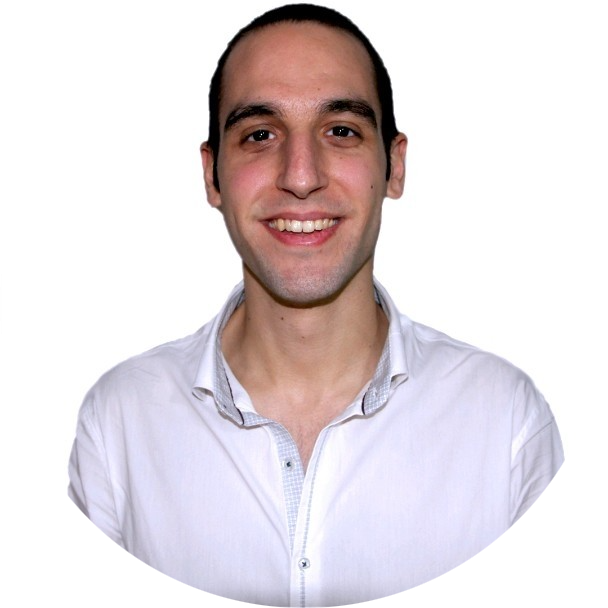
\includegraphics[width=\textwidth]{logos/circle.png}}
  \end{minipage}
  \hspace{0.01\textwidth}
  \begin{minipage}[t]{0.18\textwidth} 
    \small
    \textbf{Mario Bifulco} \\

    \textbf{Email:} \href{mario.bifulco@edu.unito.it}{mario.bifulco@edu.unito.it} \\
    \textbf{LinkedIn:} \href{https://www.linkedin.com/in/mario-bifulco/}{\url{linkedin.com/in/mario-bifulco/}} \\
    \textbf{GitHub:} \href{https://github.com/TheFlonet/qsvm4sentanalysis}{TheFlonet/qsvm4sentanalysis}
  \end{minipage}
  \hspace{0.01\textwidth}
  \begin{minipage}[t]{0.15\textwidth}
    \small 
    \textbf{Luca Roversi} \\

    \textbf{Email:} \href{luca.roversi@unito.it}{luca.roversi@unito.it} \\
    \textbf{Website:} \href{di.unito.it/~rover}{\url{di.unito.it/~rover}} \\
    \textbf{ORCID:} \href{https://orcid.org/0000-0002-1871-6109}{0000-0002-1871-6109}
  \end{minipage}
}

% ====================
% Logo (optional)
% ====================

\logoleft{
\includegraphics[height=3.5cm]{logos/logo-unito-orizz-neg.png}}
\logoright{
\includegraphics[height=3.5cm]{logos/EQAI-2024-logo.png}}

% ====================
% Body
% ====================

\begin{document}

\begin{frame}[t,fragile]
\begin{columns}[t]

\begin{column}{\colwidth}
  \begin{block}{Abstract}
    We first experiment with applying a hybrid classical-quantum classifier (HCQC) for sentiment analysis and compare it to the classical classifier and the Transformer architecture. 
    We find that HCQC is worse than Transformer in classification, but takes much less time to converge to a good solution. 
    Secondly, the work explores how to address a bottleneck of HCQC. 
    The results show how effective HCQCs can be developed, making greater use of the quantum component.
  \end{block}

  \begin{block}{Quantum Support Vector Machine for Sentiment Analysis}
    In this work, we explored the potential of \textbf{Adiabatic Quantum Computing (AQC)} applied to \textbf{Natural Language Processing (NLP)}, with a specific focus on \textbf{Binary Sentiment Analysis (BSA)}. 
    To achieve this, we undertook the following steps:

    \begin{enumerate} 
      \item Selected the TweetEval dataset\cite{TweetEval}; 
      \item Transformed the text into vectors using SentenceBert\cite{SentenceBert}; 
      \item Encoded the \textbf{Support Vector Machine (SVM)} problem using the hybrid solvers provided by D-Wave; 
      \item Assessed the quality of the proposed solution by comparing it with an implementation of SVM on classical architecture and the Transformer model RoBERTa\cite{roberta}. 
    \end{enumerate}

    The following are the results obtained, where D-Wave represents the quantum solution, RoBERTa is the Transformer architecture, and CPLEX is the classical implementation of SVM.

    \begin{figure}[h!]
      \centering
      \begin{minipage}{0.3\textwidth}
          \centering
          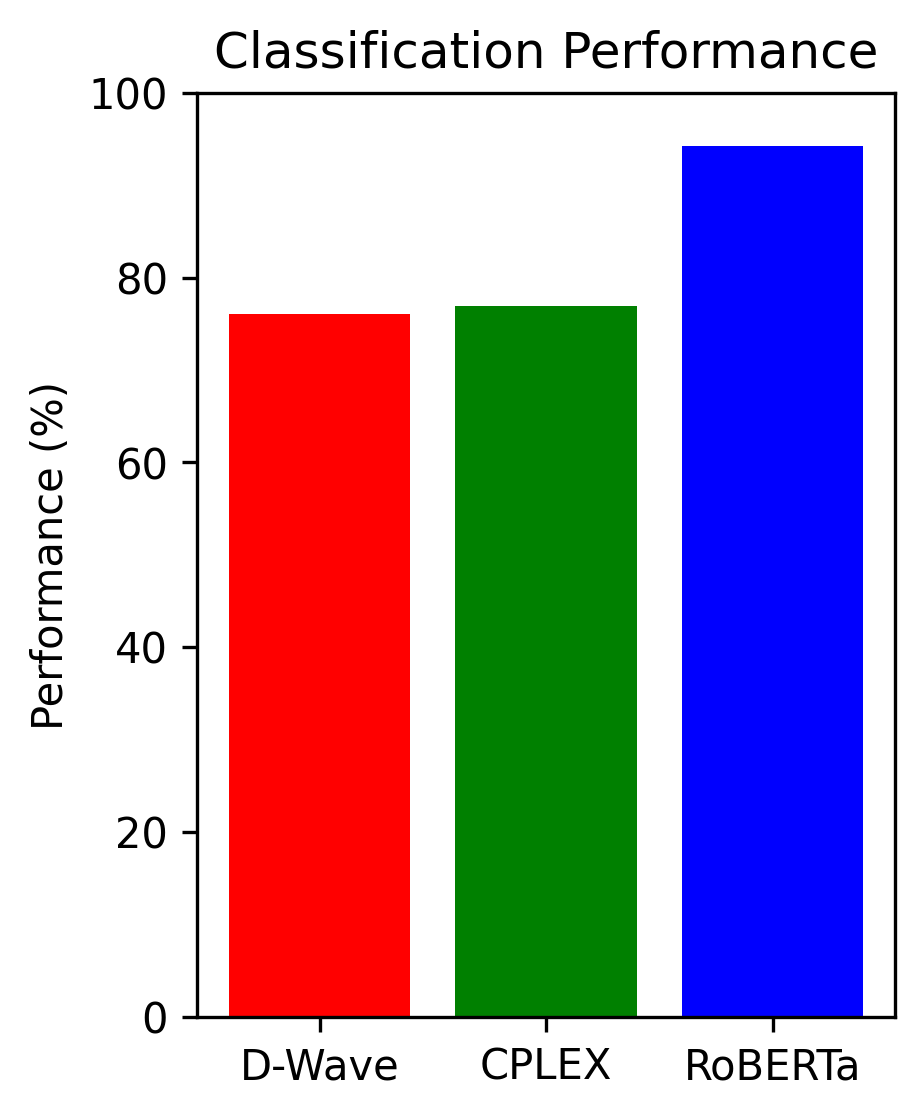
\includegraphics[height=0.15\textheight]{logos/performance.png}
      \end{minipage}%
      \hfill
      \begin{minipage}{0.65\textwidth}
        \begin{alertblock}{Classification Performance}
          The classification conducted by RoBERTa is significantly better, although the results of both CPLEX and D-Wave are also well above random guesses.
          
          The slight difference between the solution obtained with CPLEX and that with D-Wave may be due to some limitations of the current hybrid solvers, which restricted the domain of the optimisation variables from real numbers to integers.
        \end{alertblock}
      \end{minipage}
    \end{figure}

    \begin{figure}[h!]
      \centering
      \begin{minipage}{0.65\textwidth}
        \begin{alertblock}{Training Time}
          The time required by D-Wave to find an optimal assignment is 60\% less than that of CPLEX. 

          Although not available, it is reasonable to expect an even better result if compared to the time required by RoBERTa, which we can fairly expect to amount to several hours of training on high-performance machines.
        \end{alertblock}
      \end{minipage}%
      \hfill
      \begin{minipage}{0.3\textwidth}
          \centering
          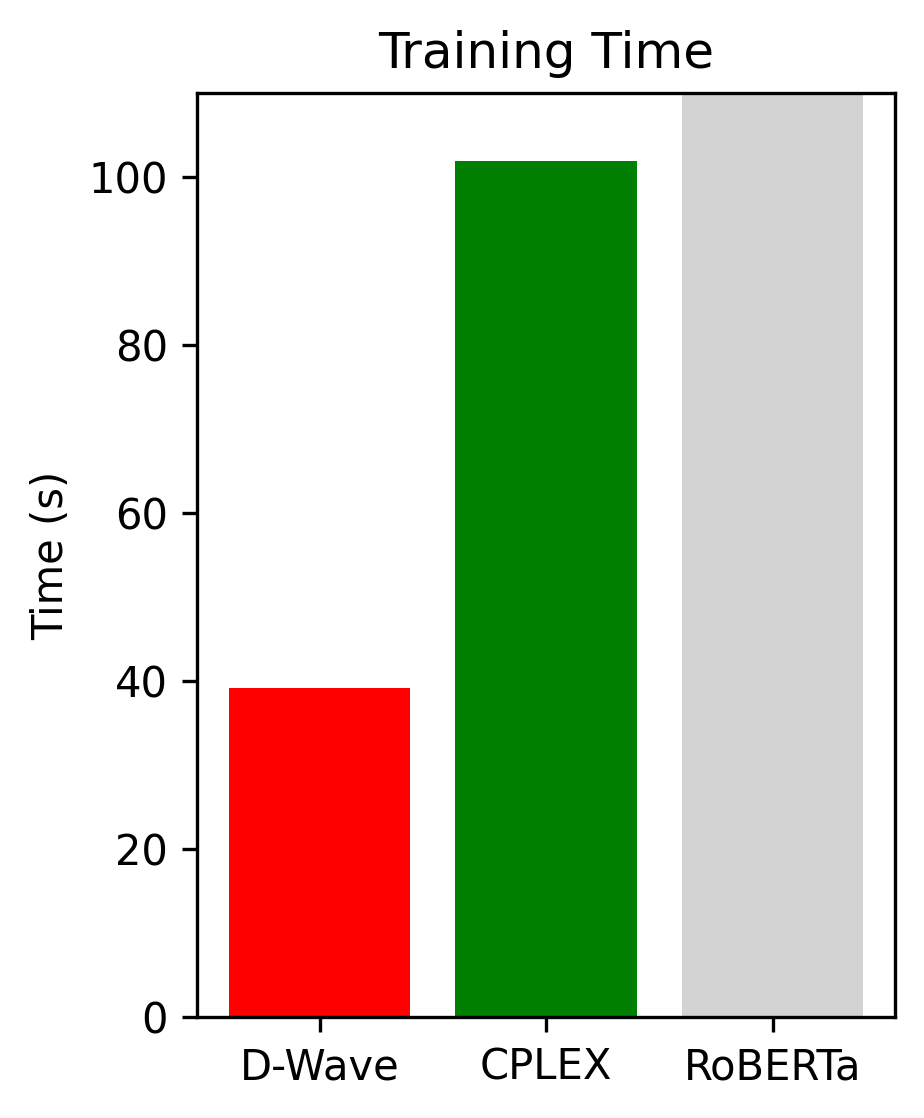
\includegraphics[height=0.15\textheight]{logos/training.png}
      \end{minipage}
    \end{figure}

    \begin{figure}[h!]
      \centering
      \begin{minipage}{0.3\textwidth}
          \centering
          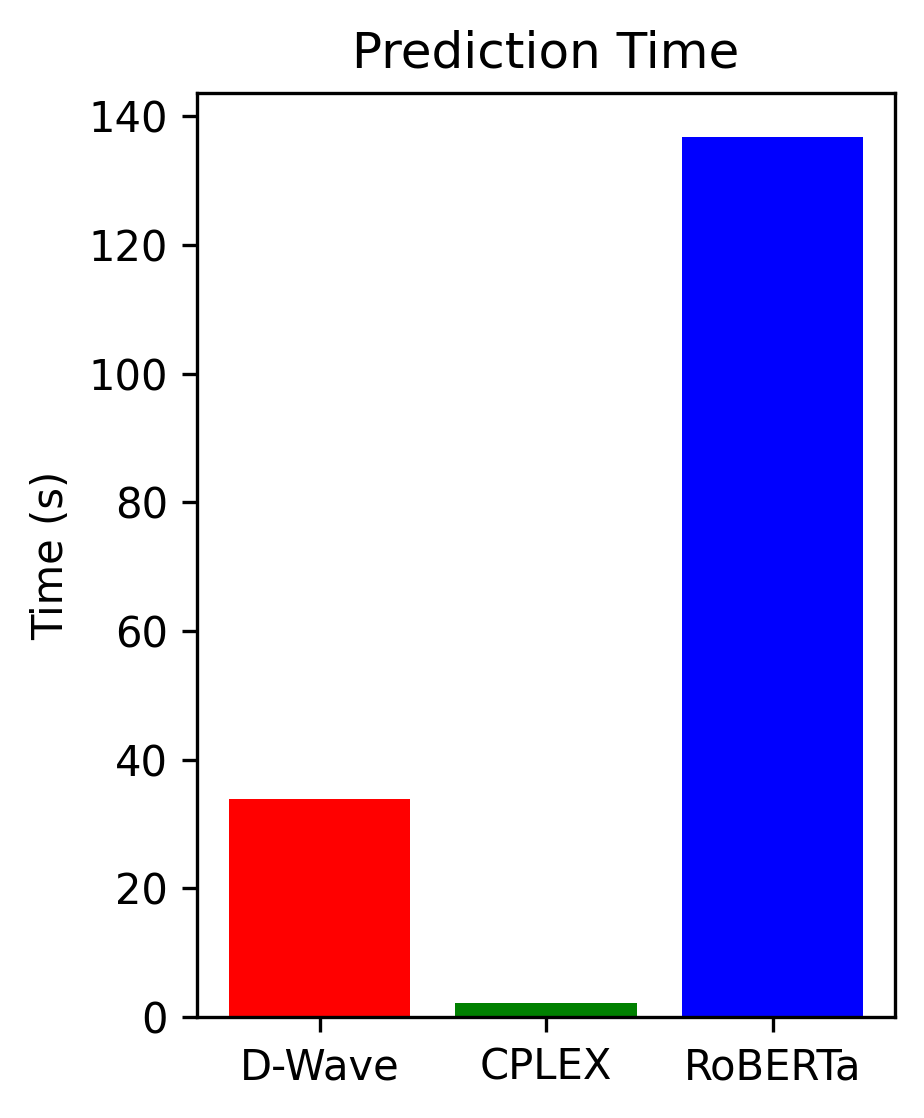
\includegraphics[height=0.15\textheight]{logos/prediction.png}
      \end{minipage}%
      \hfill
      \begin{minipage}{0.65\textwidth}
        \begin{alertblock}{Prediction Time}
          The complexity of RoBERTa architecture also affects the time required for prediction.

          The higher time required by D-Wave is due to the solving methodology, which returns a set of optimal solutions. 
          For each of them, a model is created to apply a majority vote to establish the class in inference. 

          Since no advantages emerge from using several models, it is possible to use only one of the optimal assignments, reducing the time to values comparable to those of CPLEX.
        \end{alertblock}
      \end{minipage}
    \end{figure}
  \end{block}

  \begin{block}{Maximizing Quantum Boost} 
    The default hybrid solver proposed by D-Wave appears to make only marginal use of the QPU, with an average contribution of just \textbf{0.08\%}. 
    To achieve a greater performance boost, we attempted to run the problem directly on the QPU, bypassing the opaque workflow associated with the proprietary technology of D-Wave’s hybrid solvers.

    Transforming the SVM problem to be solvable directly by the QPU requires a series of steps, the only one impacting the complexity of the procedure being the calculation of the minor embedding\cite{MEdwave}.

    \begin{figure}[h!]
      \centering
      \begin{minipage}{0.55\textwidth}
        \begin{alertblock}{Scalability Problem}
          Empirically, we identify a sweet spot for problems with 32 variables.
          
          Beyond this size, the time required to find the minor graph can become dominant compared to the time needed to solve the problem.

          Additionally, the number of qubits required to represent the problem graph becomes incompatible with the current QPU sizes (approximately 5600 qubits).
        \end{alertblock}
      \end{minipage}%
      \hfill
      \begin{minipage}{0.4\textwidth}
          \centering
          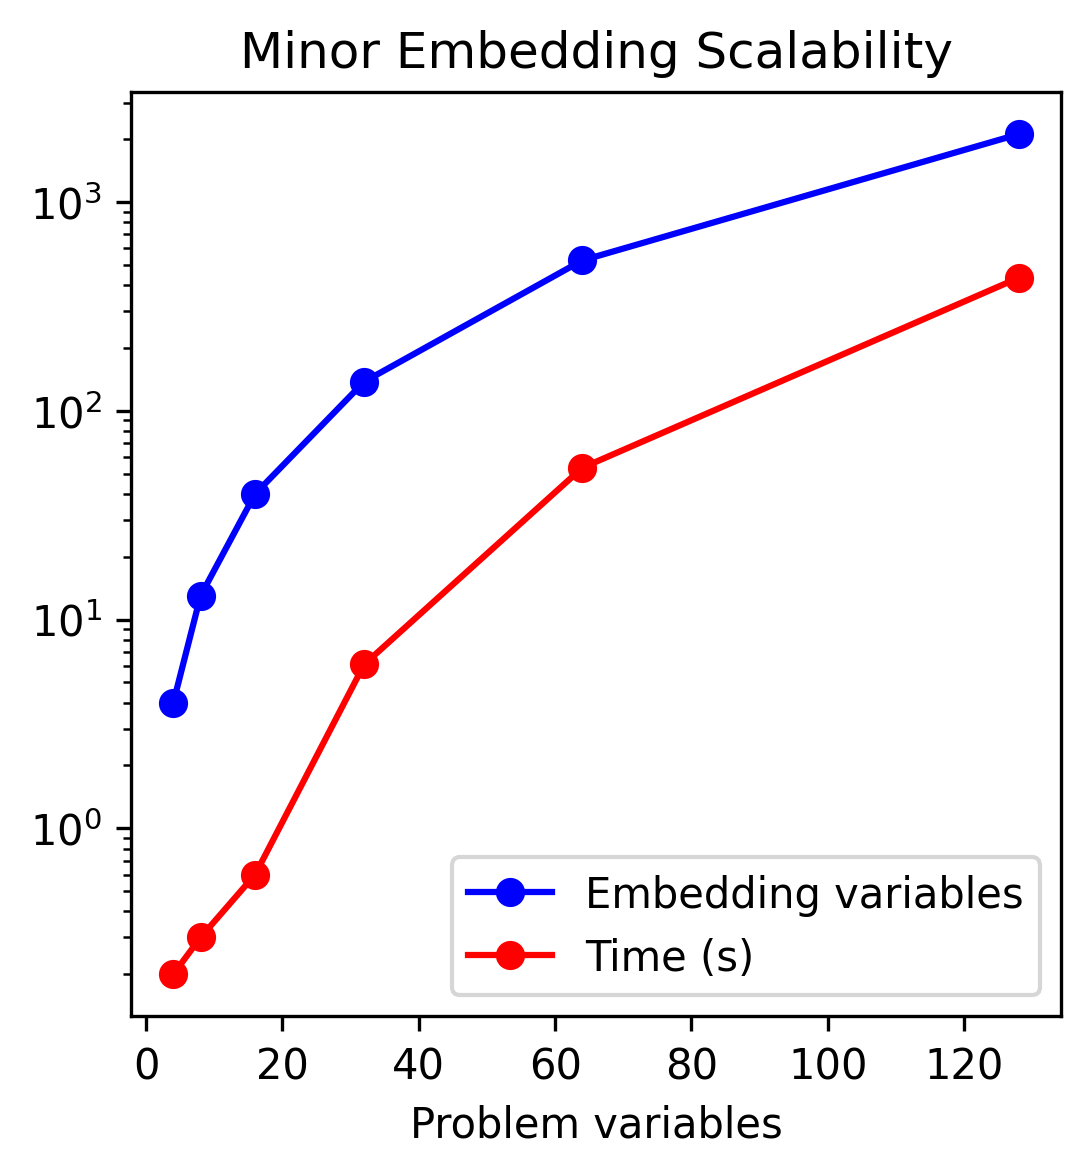
\includegraphics[height=0.15\textheight]{logos/embedding_search_time.png}
      \end{minipage}
    \end{figure}
  \end{block}
\end{column}

\separatorcolumn

\begin{column}{\colwidth}
  \begin{block}{Homebrewing a Hybrid Solver}
    Given the practical impossibility of using the QPU directly, we investigate how to design a hybrid solver, called \texttt{QSplit}, to increase the use of the QPU, based on a quite simple algebraic technique that decomposes QUBO problems into smaller chunks. 
    Sufficiently small problems can be solved by mapping them on the QPU, eventually aggregating the results. This technique is of general application, not limited to QUBO instances we get from SVM.

    \begin{figure}[h!]
      \centering
      \begin{minipage}{0.55\textwidth}
        Given any QUBO matrix we recursively divide it into four parts as in Figure \ref{fig:qubo}:
        \begin{enumerate}
            \item $\operatorname{ULs}$ and $\operatorname{BRs}$ are themselves QUBO matrices operating on a partition of the optimization variables;
            \item $\operatorname{UR}$ is not guaranteed to be upper triangular, as required by a QUBO instance, but it retains the information linking the partitions $\operatorname{UL}_0$, $\operatorname{BL}_0$ and $\operatorname{UR}_0$, $\operatorname{BR}_0$ of the variables and we can safely transform it into an upper triangular matrix, namely a QUBO instance;
            \item $\emptyset$ is a matrix composed entirely of zeros, so we ignore it.
        \end{enumerate}

        The recursive subdivision can continue until the matrices reach a predetermined size, namely Stopping dimension.
      \end{minipage}%
      \hfill
      \begin{minipage}{0.4\textwidth}
        \centering
        \begin{tikzpicture}
            \draw (0,0) rectangle (8,8);
        
            \draw (0,4) -- (8,4);
            \draw (4,0) -- (4,8);
            \node at (2,2) {$\emptyset$};
            
            \draw (0,6) -- (4,6);
            \draw (2,8) -- (2,4);
            \node at (1,5) {$\emptyset$};
        
            \draw (4,2) -- (8,2);
            \draw (6,4) -- (6,0);
            \node at (5,1) {$\emptyset$};
    
            \draw (4,6) -- (8,6);
            \draw (6,4) -- (6,8);
            \node at (5,5) {$\emptyset$};
        
            \draw[decorate,decoration={brace,amplitude=10pt}] (8,8) -- (8,4) node [black,midway,xshift=25pt] {$\operatorname{UR}_0$};
            \node at (3,7) {$\operatorname{UR}_1'$};
            \node at (7,7) {$\operatorname{UR}_1''$};
            \node at (7,3) {$\operatorname{UR}_1'''$};
    
            \draw[decorate,decoration={brace,amplitude=10pt,mirror}] (0,8) -- (0,4) node [black,midway,xshift=-25pt] {$\operatorname{UL}_0$};
            \node at (1,7) {$\operatorname{UL}_1'$};
            \node at (5,7) {$\operatorname{UL}_1''$};
            \node at (5,3) {$\operatorname{UL}_1'''$};
    
            \draw[decorate,decoration={brace,amplitude=10pt}] (8,4) -- (8,0) node [black,midway,xshift=25pt] {$\operatorname{BR}_0$};
            \node at (3,5) {$\operatorname{BR}_1'$};
            \node at (7,5) {$\operatorname{BR}_1''$};
            \node at (7,1) {$\operatorname{BR}_1'''$};

            \draw[decorate,decoration={brace,amplitude=10pt,mirror}] (0,4) -- (0,0) node [black,midway,xshift=-25pt] {$\operatorname{BL}_0$};
        \end{tikzpicture}
        \caption{Two steps of recursive decomposition}
        \label{fig:qubo}
      \end{minipage}
    \end{figure}

    \begin{exampleblock}{Example of one recursive step}
      Let us assume that we have classifications offered by $\operatorname{UL}_1'$, $\operatorname{UR}_1'$, $\operatorname{BR}_1'$. 

      \begin{enumerate}
        \item $\operatorname{UL}_1'$ and $\operatorname{BR}_1'$ are combined to generate conflict-free initial assignments called $\operatorname{S_1}$;
        \item The solutions from $\operatorname{S_1}$ and those obtained from $\operatorname{UR}_1'$ are combined by searching for compatible assignments and marking conflicting variables;
        \item From the conflicting values, a QUBO problem is extracted, considering only the rows and columns associated with these variables, which is again solved via QPU;
        \item From the set of possible assignments obtained by solving conflicting classifications, duplicates are removed and only the $k$ most promising assignments are retained. 
      \end{enumerate}
    \end{exampleblock}

    We tested \texttt{QSplit} with problems from 128 variables, and the data collected showed the following behaviour \textbf{when decreasing the Stopping dimension}.

    \begin{figure}[h!]
      \centering
      \begin{minipage}{0.6\textwidth}
        \centering
        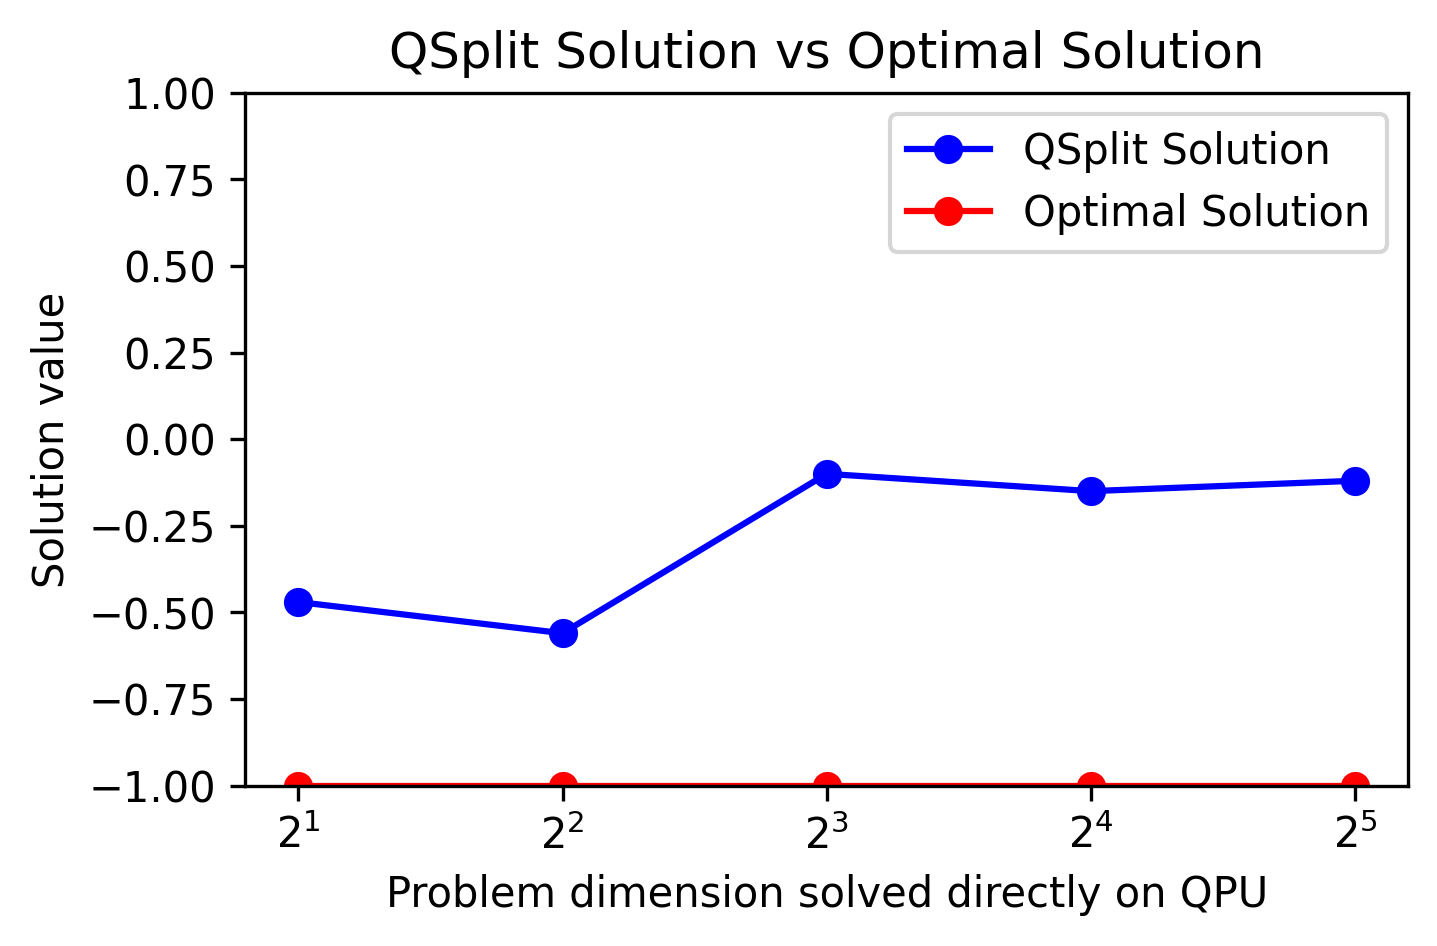
\includegraphics[height=0.15\textheight]{logos/sol.png}
      \end{minipage}%
      \hfill
      \begin{minipage}{0.35\textwidth}
        \begin{alertblock}{\texttt{QSplit} Performance}
          The quality of the solution improves, with the error decreasing from 45\% to 25\%.
        \end{alertblock}
      \end{minipage}
    \end{figure}

    \begin{figure}[h!]
      \centering
      \begin{minipage}{0.35\textwidth}
        \begin{alertblock}{\texttt{QSplit} Execution Time}
          The time required by \texttt{QSplit} increases, ranging from requiring 40\% less time compared to direct resolution to requiring 50\% more time.
        \end{alertblock}
      \end{minipage}%
      \hfill
      \begin{minipage}{0.6\textwidth}
          \centering
          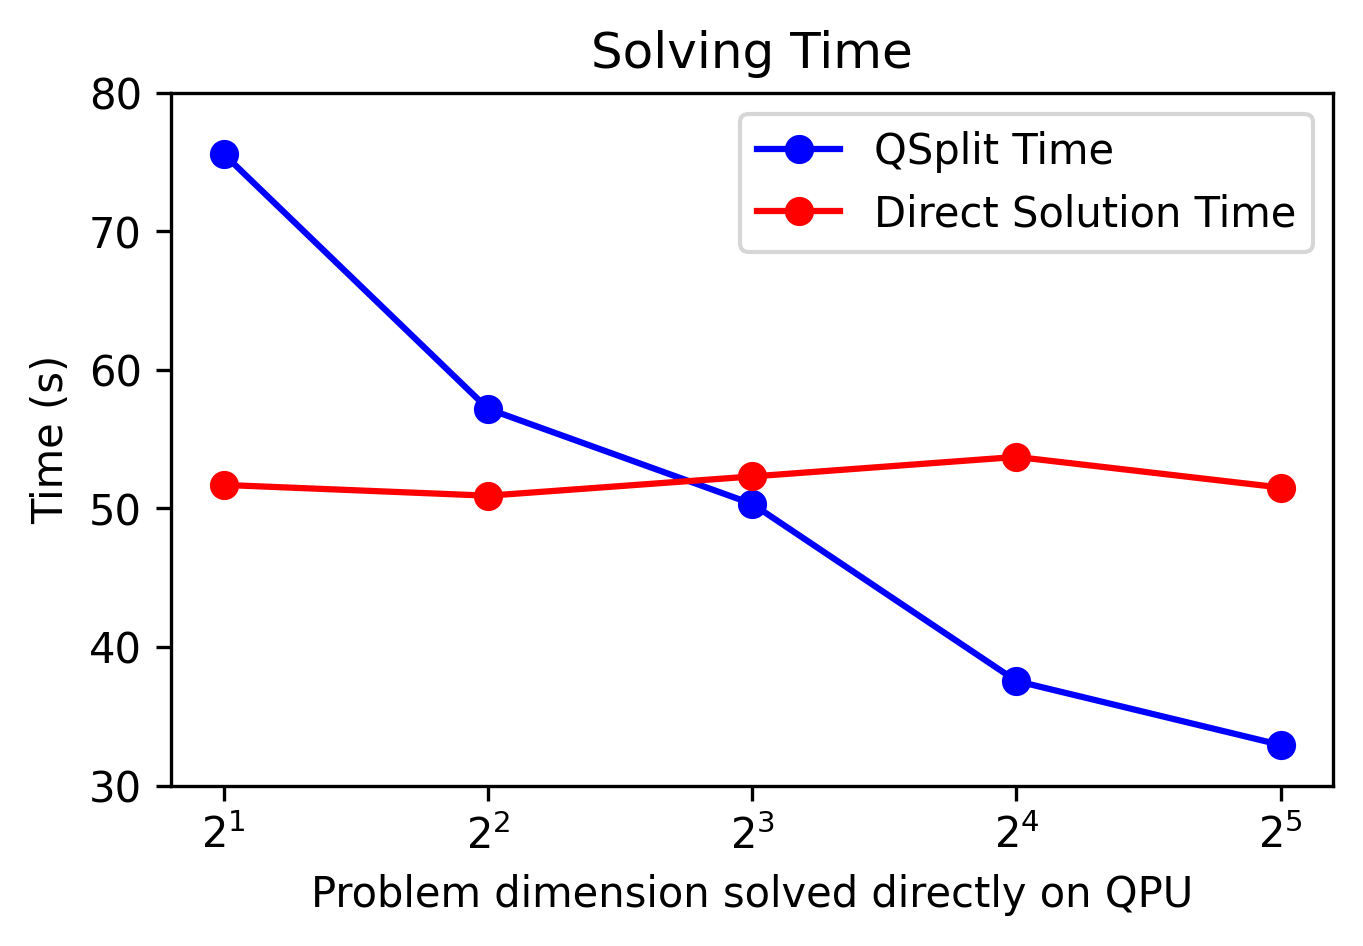
\includegraphics[height=0.15\textheight]{logos/time.png}
      \end{minipage}
    \end{figure}
  \end{block}

  \begin{block}{Conclusion}
    Our investigation contributes to giving evidence that quantum computing can bring tangible benefits over traditional methods to solve optimization problems. 
    In many application scenarios, large computational resources are not available, such as in personal computers or embedded systems. 
    In these situations, hybrid solvers such as the one we have presented are good candidates to allow for a good approximation of results while significantly reducing complexity and computational power.

    \texttt{QSplit} presents an alternative method for handling large QUBO problems to those found in the literature\cite{subqubo2}. 
    The assignment produced can be improved by implementing more refined problem partitioning strategies\cite{bnb}, or by creating work pipelines capable of using a set of methods for finding the optimal assignment\cite{dwavehybrid}.
  \end{block}

  \begin{block}{Bibliography}
    \begin{thebibliography}{10}
      \bibitem{TweetEval} Rosenthal Sara et al., ``SemEval-2017 task 4: Sentiment analysis in Twitter''.
      \bibitem{SentenceBert} Reimers Nils et al., ``Sentence-BERT: Sentence Embeddings using Siamese BERT-Networks''.
      \bibitem{roberta} CardiffNLP, ``Twitter-roBERTa-base for Sentiment Analysis''.
      \bibitem{MEdwave} Jun Cai et al., ``A practical heuristic for finding graph minors''.
      \bibitem{subqubo2} Tameem Albash et al., ``Solving large optimization problems with restricted quantum annealers''.
      \bibitem{bnb} Sanavio Claudio et al., ``Hybrid Classical–Quantum Branch-and-Bound Algorithm for Solving Integer Linear Problems''.
      \bibitem{dwavehybrid} Michael Booth et al., ``Partitioning Optimization Problems for Hybrid Classical/Quantum Execution''.
    \end{thebibliography}
  \end{block}
\end{column}

\end{columns}
\end{frame}

\end{document}
